\documentclass[12pt, a4paper]{article}

\usepackage{polski}
\usepackage[utf8]{inputenc}
\usepackage{amsmath}
\usepackage{amsfonts}
\usepackage{graphicx}
\usepackage[margin=0.7in]{geometry}
\usepackage{url}
\usepackage[hidelinks]{hyperref}
\usepackage{enumitem}
\usepackage{subcaption}
\usepackage{float}

\usepackage{titlesec}

\providecommand{\tightlist}{%
  \setlength{\itemsep}{0pt}\setlength{\parskip}{0pt}}

\begin{document}
\setlength{\parindent}{0pt}
\begin{titlepage}
    \centering
    \vspace{20cm}
    {\huge\bfseries TinyAd \unskip\strut\par}
    {\huge\bfseries Dokumentacja końcowa \unskip\strut\par}
    \vspace{1cm}
    {\Large\itshape Rafał Kulus (Lider), \\Damian Kolaska, \\Kamil Przybyła \unskip\strut\par}
    \vspace{1cm}
    \href{https://bitbucket.org/BlueAlien99/tinyad}{https://bitbucket.org/BlueAlien99/tinyad}

    \vfill
    
    {\large \today\par}
\end{titlepage}
\tableofcontents
\clearpage

\hypertarget{treux15bux107-zadania}{%
\section{Treść zadania}\label{treux15bux107-zadania}}

W systemie pracuje stacja zarządzająca i zbiór (do kilkudziesięciu
tysięcy) sterowników paneli reklamowych. Stacja multicastowo dystrybuuje
treści i harmonogramy ich wyświetlania. Harmonogram określa okresy
wyświetlania i czas przechowywania. Sterowniki unicastowo raportują swój
stan i zgłaszają błędy. Błąd w transmisji multicastowej obsługiwany jest
retransmisją multi- lub unicastową w zależności od liczby otrzymanych
komunikatów NAK. System ma pracować w prywatnej sieci IPv6. Stacja
zarządzająca może wysyłać unicastowo ważne treści informacyjne do
natychmiastowego wyświetlenia przez wybrane sterowniki. Należy też
zaprojektować moduł do Wireshark umożliwiający wyświetlanie i analizę
zdefiniowanych komunikatów.

\hypertarget{format-plikuxf3w}{%
\section{Format plików}\label{format-plikuxf3w}}

\hypertarget{konfiguracja-dla-paneli}{%
\subsection{Konfiguracja dla paneli}\label{konfiguracja-dla-paneli}}

\texttt{panel\_name} i \texttt{tags} są opcjonalne i służą do
identyfikowania paneli, w celu wyświetlenia ważnych treści. Są wysyłane
do stacji zarządzającej podczas rejestrowania panelu. Domyślna nazwa i
lokalizacja pliku to \texttt{./config.conf}.

\begin{verbatim}
server_ip=fe80::1234
panel_name=Lobby Front
tags=[oled][huge][orange apricot]
\end{verbatim}

\hypertarget{harmonogram}{%
\subsection{Harmonogram}\label{harmonogram}}

\texttt{expire}, \texttt{weekday}, \texttt{hour} są opcjonalne. W
przypadku braku \texttt{expire}, zawartość nigdy nie wygaśnie. W
przypadku braku pozostałych dwóch pól, zawartość będzie wyświetlana
niezależnie od dnia tygodnia i / lub godziny. Pierwszeństwo ma pierwsza
zawartość, która spełnia wszystkie warunki. Dni tygodnia są indeksowane od 1.

\begin{verbatim}
file=./img.jpg
expire=2021.05.15 19:30
weekday=[1][2][3]
hour=[05:30-08:30][15:00-19:00]
---
file=./vids/video.mp4
expire=2021.06.30 00:00
\end{verbatim}

\hypertarget{interfejs-uux17cytkownika}{%
\section{Interfejs użytkownika}\label{interfejs-uux17cytkownika}}

\hypertarget{stacja-zarzux105dzajux105ca}{%
\subsection{Stacja zarządzająca}\label{stacja-zarzux105dzajux105ca}}

Stacja zarządzająca posiada prosty CLI.

Dostępne polecenia: 

\begin{enumerate}
\def\labelenumi{\arabic{enumi}.}
\tightlist
\item \texttt{schedule\ ./my\_sched.sched} \\
Spowoduje rozesłanie nowego harmonogramu i wymaganych plików do paneli.\\ \texttt{./my\_sched.sched} to ścieżka do pliku zawierającego harmonogram.
\item \texttt{panic\ ./emergency.mkv\ -\/-name\ "Lobby\ Front"}
\item \texttt{panic\ ./emergency.mkv\ -\/-tags\ {[}oled{]}{[}huge{]}}\\
Spowoduje wysłanie ważnych treści do paneli, których nazwa to
\texttt{Lobby\ Front} lub które posiadają co najmniej jeden z podanych
tagów. Ważne treści będą wyświetlane tak długo, aż panel nie otrzyma
nowego harmonogramu poleceniem \texttt{schedule}
\item \texttt{bye} \\
Spowoduje wyłączenie stacji zarządzającej
\item \texttt{top\ 10} \\
Wyświetlenie 10 ostatnich linii logów.
\end{enumerate}

\hypertarget{panele}{%
\subsection{Panele}\label{panele}}

Panele nie posiadają interfejsu użytkownika. Wszystkie potrzebne
informacje są wczytywane z prostego pliku konfiguracyjnego.

\hypertarget{pozostaux142e-zaux142oux17cenia-funkcjonalne}{%
\section{Pozostałe założenia funkcjonalne}\label{pozostaux142e-zaux142oux17cenia-funkcjonalne}}

Proces uruchomienia paneli powinien się ograniczyć tylko i wyłącznie do
startu aplikacji klienta, która sama wykona wszystkie wymagane
czynności, aby panel mógł zacząć wyświetlać zawartość.

Po udanej rejestracji panelu w stacji zarządzającej zostanie do niego
natychmiastowo wysłany adres multicast do nasłuchiwania nowych harmonogramów.

\hypertarget{zaux142oux17cenia-niefunkcjonalne}{%
\section{Założenia niefunkcjonalne}\label{zaux142oux17cenia-niefunkcjonalne}}

Stacje zarządzające i panele powinny sobie radzić ze wszystkimi
przewidzianymi błędami, aby zapewnić nieprzerwaną pracę, stabilność i
niezawodność, w szczególności błędy transmisji danych nie powinny
uniemożliwić poprawnego działania systemu.

\hypertarget{przypadki-uux17cycia}{%
\section{Przypadki użycia}\label{przypadki-uux17cycia}}

\hypertarget{rejestracja-panelu-reklamowego}{%
\subsection{Rejestracja panelu reklamowego}\label{rejestracja-panelu-reklamowego}}

\begin{enumerate}
\def\labelenumi{\arabic{enumi}.}
\tightlist
\item
  Użytkownik uruchamia panel reklamowy (opcjonalnie podając plik
  konfiguracyjny)
\item
  Panel rejestruje się, wysyłając komunikat stacji zarządzającej
\item
  Panel otrzymuje adres multicast do nasłuchiwania nowych harmonogramów
\end{enumerate}

\hypertarget{zarzux105dzanie-harmonogramem-oraz-wyux15bwietlanymi-treux15bciami}{%
\subsection{Zarządzanie harmonogramem oraz wyświetlanymi treściami}\label{zarzux105dzanie-harmonogramem-oraz-wyux15bwietlanymi-treux15bciami}}

\begin{enumerate}
\def\labelenumi{\arabic{enumi}.}
\tightlist
\item
  Użytkownik, za pośrednictwem stacji zarządzającej, modyfikuje
  informacje o harmonogramie lub treściach
\item
  Stacja zarządzająca wysyła aktualne dane do paneli
\item
  Panele wyświetlają treści zgodnie z otrzymanym harmonogramem
\end{enumerate}

\hypertarget{zlecenie-natychmiastowego-wyux15bwietlenia-informacji}{%
\subsection{Zlecenie natychmiastowego wyświetlenia informacji}\label{zlecenie-natychmiastowego-wyux15bwietlenia-informacji}}

\begin{enumerate}
\def\labelenumi{\arabic{enumi}.}
\tightlist
\item
  Użytkownik, za pośrednictwem stacji zarządzające, zleca natychmiastowe
  wyświetlenie informacji podanej podgrupie paneli
\item
  Stacja zarządzająca wysyła treść do natychmiastowego wyświetlenia
\item
  Panele wyświetlają żądaną treść, ignorując treści wynikające z
  harmonogramu
\end{enumerate}

\hypertarget{obsux142uga-bux142ux119duxf3w}{%
\section{Obsługa błędów}\label{obsux142uga-bux142ux119duxf3w}}

\hypertarget{brak-harmonogramu}{%
\subsection{Brak harmonogramu}\label{brak-harmonogramu}}

Panel wyświetlał będzie informację o braku harmonogramu.

\hypertarget{bledny-harmonogram}{%
\subsection{Błędny harmonogram}\label{bledny-harmonogram}}

Jeśli harmonogram zawiera błędy składniowe lub opisane w nim pliki nie istnieją, błąd zostanie zgłoszony i harmonogram nie zostanie przesłany do panelu.

\hypertarget{brak-pliku-konfiguracyjnego}{%
\subsection{Brak pliku konfiguracyjnego}\label{brak-pliku-konfiguracyjnego}}

Wyświetlenie odpowiedniej informacji zwrotnej użytkownikowi i zamknięcie
aplikacji.

\hypertarget{bux142ux105d-transmisji-danych}{%
\subsection{Błąd transmisji danych}\label{bux142ux105d-transmisji-danych}}

W przypadku, gdy w wyniku błędu sieciowego, jeden lub więcej pakietów
zostanie zagubionych, odbiorca wyśle komunikat z prośbą o ponowne
przesłanie brakujących segmentów.

\hypertarget{ux15brodowisko-programistyczne}{%
\section{Środowisko programistyczne}\label{ux15brodowisko-programistyczne}}

Projekt został zrealizowany na systemie operacyjnym Ubuntu 20.04 LTS,
w języku C++17. Do testów została wykorzystana biblioteka GoogleTest, a
do debugowania programy gdb, valgrind oraz Wireshark. Do budowania
projektu użyto CMake oraz g++. Do logowania skorzystaliśmy z
biblioteki Loguru (\href{https://github.com/emilk/loguru}{https://github.com/emilk/loguru}).

\hypertarget{architektura}{%
\section{Architektura}\label{architektura}}

\hypertarget{stacja-zarzux105dzajux105ca-1}{%
\subsection{Stacja zarządzająca}\label{stacja-zarzux105dzajux105ca-1}}

\begin{center}
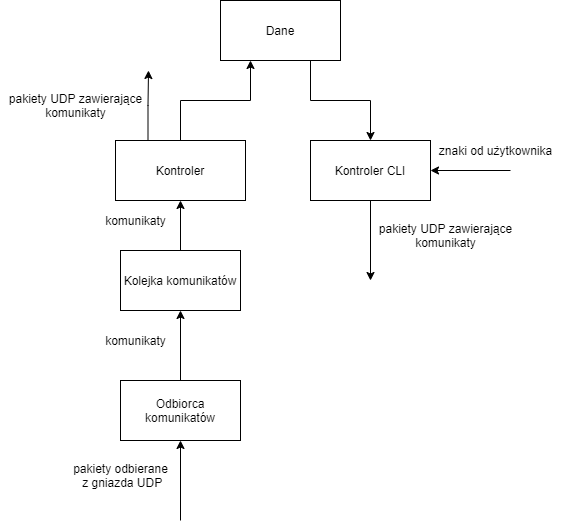
\includegraphics[width=0.55\textwidth]{server_arch.png}
\end{center}

\textbf{Odbiorca komunikatów}

Odbiera pakiety z gniazda UDP, umieszcza je w kolejce i powraca do dalszego nasłuchiwania.

\textbf{Kontroler}

Przetwarza pakiety z kolejki: deserializuje je na komunikaty, sprawdza ich poprawność i na ich podstawie podejmuje odpowiednie działania.

\textbf{Kontroler CLI}

Odbiera polecenia podawane na standardowe wejście i na ich podstawie podejmuje odpowiednie działania.

\textbf{Dane}

Wszystkie struktury danych używane przez serwer (rejestr paneli, rejestr plików).

\hypertarget{panel}{%
\subsection{Panel}\label{panel}}

\begin{center}
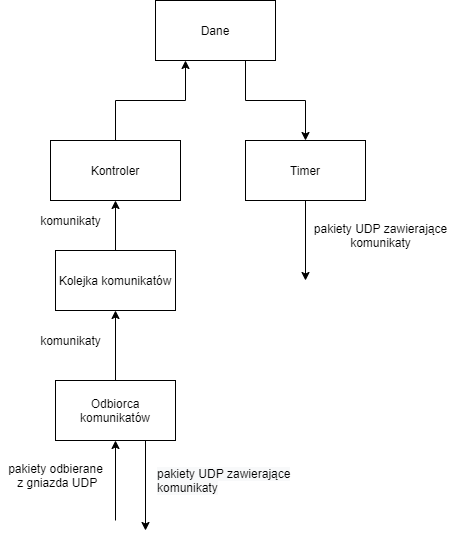
\includegraphics[width=0.55\textwidth]{client_arch.png}
\end{center}

\textbf{Odbiorca komunikatów}

Odbiera pakiety z gniazda UDP i umieszcza w kolejce i powraca do dalszego nasłuchiwania. Wysyła wiadomość typu \texttt{CONTROL\_SLOW\_DOWN\_TRANSMISSION}, jeśli nastąpi przepełnienie kolejki.

\textbf{Kontroler}

Przetwarza pakiety z kolejki: deserializuje je na komunikaty, sprawdza ich poprawność i na ich podstawie podejmuje odpowiednie działania.

\textbf{Timer}

Okresowo wysyła do stacji wiadomości typu NAK oraz \texttt{PanelHello}.

\textbf{Dane}

Wszystkie struktury danych używane przez klienta (harmonogram, konfiguracja, rejestr plików).

\hypertarget{implementacja}{%
\section{Implementacja systemu}\label{implementacja}}

W celu ułatwienia implementacji protokołu komunikacji, przygotowano klasę będącą abstrakcją nad UNIXowy interfejs do gniazd UDP (\ref{fig:class_diagram2}). Powstała również klasa symulująca wadliwe połączenie, w którym część pakietów jest losowo gubiona. Zastosowany został wzorzec fasady.

\begin{figure}[H]
\centering
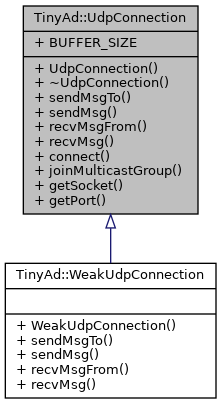
\includegraphics[width=0.15\linewidth]{class_diagram2}
\caption{Diagram klas dla fasady odpowiedzialnej za komunikację UDP}
\label{fig:class_diagram2}
\end{figure}
Wszystkie komunikaty są reprezentowane przez klasy potomne wspólnej klasy abstrakcyjnej wymagającej implementacji funkcji, która zwraca typ wiadomości (\ref{fig:class_diagram1}). Informacja ta jest wykorzystywana przy deserializacji.

\begin{figure}[H]
\centering
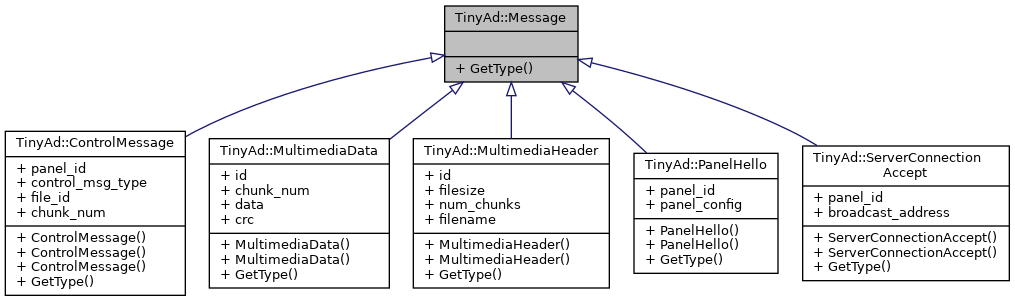
\includegraphics[width=0.9\linewidth]{class_diagram1}
\caption{Diagram klas przestawiający typy komunikatów}
\label{fig:class_diagram1}
\end{figure}
Do pozostałych klas, wykorzystanych w projekcie należą:

\begin{itemize}
\tightlist
\item \texttt{CLI} -- ułatwia tworzenie tekstowego interfejsu użytkownika
\item \texttt{ConfigBlock} -- reprezentuje blok par klucz-wartość w pliku konfiguracyjnym  (bloki oddzielone są separatorem)
\item \texttt{ConfigParser} -- parser plików konfiguracyjnych 
\item \texttt{ConfigValue} -- reprezentuje wartość odpowiadającą kluczowi w pliku konfiguracyjnym
\item \texttt{Date} (oraz inne klasy przechowujące czas)
\item \texttt{FileDeserializer} -- tworzy plik na podstawie odebranych pakietów
\item \texttt{FileSerializer} -- generuje komunikaty wykorzystywane do przesyłania danych
\item \texttt{MessageQueue} -- kolejka przechowująca odbierane pakiety z wbudowaną synchronizacją
\item \texttt{PanelConfig} -- reprezentuje plik konfiguracyjny panelu
\item \texttt{Schedule} -- reprezentuje harmonogram
\item \texttt{ScheduleEntry} -- reprezentuje pojedynczy wpis w harmonogramie
\item \texttt{Storage} -- interfejs do bazy danych (nieużywany)
\end{itemize}

\begin{figure}[H]
\centering
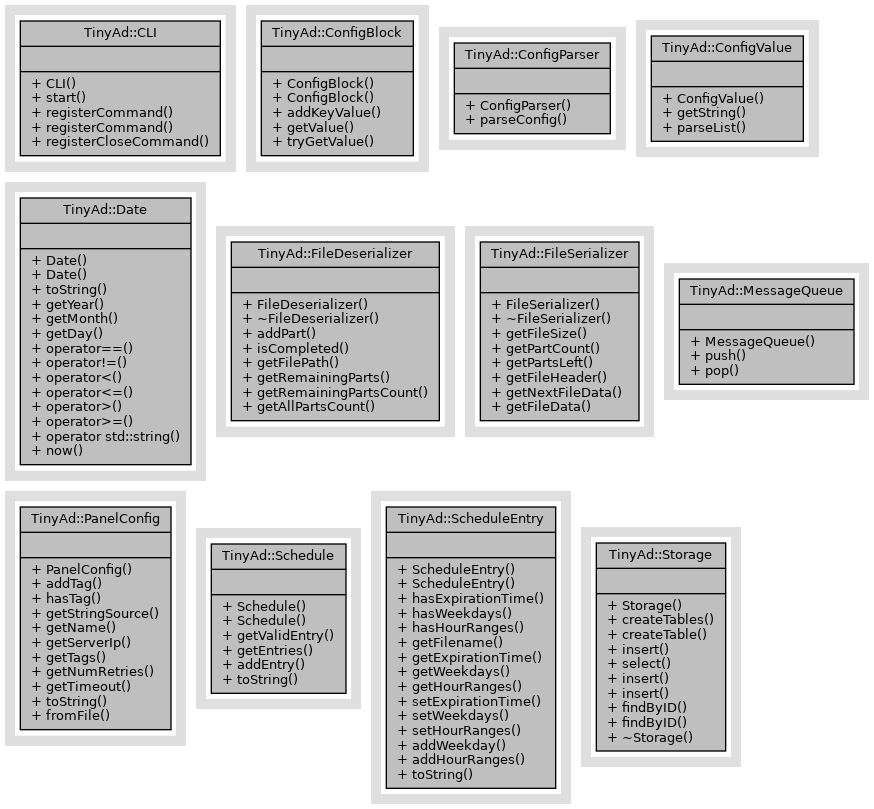
\includegraphics[width=0.8\linewidth]{class_diagram3}
\caption{Pozostałe klasy wykorzystywane w projekcie}
\label{fig:class_diagram3}
\end{figure}


\hypertarget{komunikaty}{%
\section{Komunikaty}\label{komunikaty}}

\hypertarget{struktura-komunikatow}{%
\subsection{Struktura komunikatów}\label{struktura-komunikatow}}

\hypertarget{multimedia-header}{%
\subsubsection{MultimediaHeader}\label{multimedia-header}}

Komunikat wysyłany przez stację zarządzającą. Zawiera metadane pliku, który ma zostać przesłany.

\begin{verbatim}
struct MultimediaHeader {
    std::string id;
    uint32_t filesize;
    uint32_t num_chunks;
    std::string filename;
};
\end{verbatim}

\begin{itemize}
\tightlist
    \item \texttt{id} -- unikalny identyfikator pliku
    \item \texttt{filesize} -- rozmiar pliku
    \item \texttt{num\_chunks} -- liczba fragmentów, na które podzielony zostanie plik 
    \item \texttt{filename} -- nazwa pliku
\end{itemize}

\hypertarget{multimedia-data}{%
\subsubsection{MultimediaData}\label{multimedia-data}}

Zawiera dane stanowiące fragment pliku. Wysyłane przez stację zarządzającą i odbierane przez panele.

\begin{verbatim}
struct MultimediaData {
    std::string id;
    uint32_t chunk_num;
    std::string data;
    uint32_t crc;
};
\end{verbatim}

\begin{itemize}
\tightlist
    \item \texttt{id} -- unikalny identyfikator pliku
    \item \texttt{chunk\_num} -- numer fragmentu pliku
    \item \texttt{data} -- dane pliku 
    \item \texttt{crc} -- suma kontrolna
\end{itemize}

\hypertarget{control-message}{%
\subsubsection{ControlMessage}\label{control-message}}

Komunikat służący do transmisji wiadomości kontrolnych. Są wysyłane zarówno przez stację jak i przez panele.

\begin{verbatim}
struct ControlMessage {
    std::string panel_id;
    ControlMsgType control_msg_type;
    std::string file_id;
    int chunk_num;
};
\end{verbatim}

\begin{itemize}
\tightlist
    \item \texttt{panel\_id} -- unikalny identyfikator panelu
    \item \texttt{control\_msg\_type} -- typ wiadomości kontrolnej
    \item \texttt{file\_id} -- unikalny identyfikator pliku
    \item \texttt{chunk\_num} -- numer fragmentu pliku
\end{itemize}

Do typów wiadomości kontrolnych należą:

\begin{itemize}
\tightlist
    \item \texttt{CONTROL\_NAK} -- komunikat informaujący o brakującym fragmencie danych pliku; wysyłany przez panel
    \item \texttt{CONTROL\_FILE\_HEADER\_REQUESTED} -- informuje o brakującym nagłówku pliku; wysyłany przez panel
    \item \texttt{CONTROL\_SLOW\_DOWN\_TRANSMISSION} -- wysyłany przez panel, gdy kolejka nieobsłużonych komunikatów się zapełni
    \item \texttt{CONTROL\_FILE\_NOT\_FOUND} -- wysyłany przez serwer, gdy pożądany plik nie istnieje 
\end{itemize}

\hypertarget{panel-hello}{%
\subsubsection{PanelHello}\label{panel-hello}}

Wysyłany przez panel w celu rejestracji w stacji zarządzającej. Służy również za keep-alive.

\begin{verbatim}
struct PanelHello {
    std::string panel_id;
    std::string panel_config;
};
\end{verbatim}

\begin{itemize}
\tightlist
    \item \texttt{panel\_id} -- unikalny identyfikator panelu
    \item \texttt{panel\_config} -- konfiguracja panelu
\end{itemize}

\hypertarget{server-connection-accept}{%
\subsubsection{ServerConnectionAccept}\label{server-connection-accept}}

Komunikat wysyłany przez serwer, jako odpowiedź na \texttt{PanelHello}.

\begin{verbatim}
struct ServerConnectionAccept {
    std::string panel_id;
    std::string broadcast_address;
};
\end{verbatim}

\begin{itemize}
\tightlist
    \item \texttt{panel\_id} -- unikalny identyfikator panelu
    \item \texttt{broadcast\_address} -- adres multicast do nasłuchiwania przez panel
\end{itemize}

\hypertarget{kodowanie-komunikatow}{%
\subsection{Kodowanie komunikatów}\label{kodowanie-komunikatow}}

Przed wysyłaniem komunikatu dodawane jest na początku pole będące liczbą 8-bitową bez znaku informujące o typie wiadomości. Informacja ta jest konieczna, aby rozróżnić typ odebranego komunikatu. Ciągi znaków poprzedzane są ich długością. 
\\
Rozmiar danych przesyłanych w komunikacie \texttt{MultimediaData} jest ograniczony do 512 bajtów. 

\hypertarget{przesyux142anie-danych}{%
\section{Przesyłanie danych}\label{przesyux142anie-danych}}


Serwer po uruchomieniu oczekuje na komunikaty \texttt{PanelHello} od paneli. Po otrzymaniu takiego komunikatu rejestruje panel. Przy zmianie harmonogramu serwer ładuje wszystkie pliki zawarte w harmonogramie i wysyła je wraz z harmonogramem do wszystkich zarejestrowanych paneli.
\\
\\
Panel po otrzymaniu nagłówka pliku rejestruje go jako aktywny. Panele posiadają oddzielny wątek sprawdzający, czy istnieją aktywne pliki, które nie zostały w całości pobrane, i wysyłający komunikaty NAK dla losowych fragmentów takich plików.



\hypertarget{pliki-multimedialne}{%
\subsection{Pliki multimedialne}\label{pliki-multimedialne}}

\begin{figure}[H]
\centering
  \begin{subfigure}[b]{0.48\linewidth}
    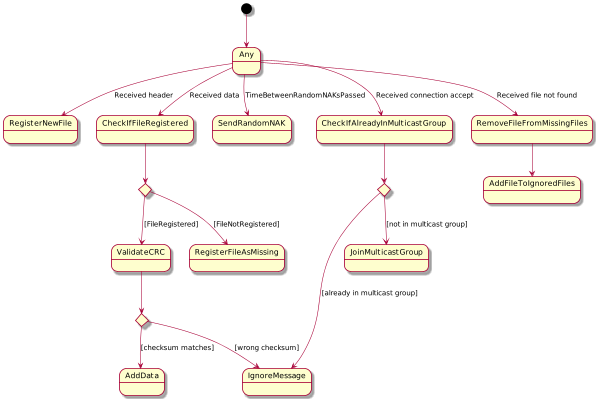
\includegraphics[width=0.7\linewidth]{client_diagram.png}
    \caption{Klient}
  \end{subfigure}
  \begin{subfigure}[b]{0.48\linewidth}
    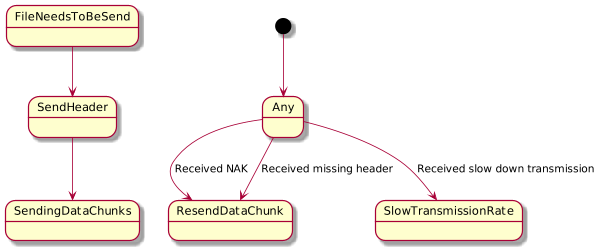
\includegraphics[width=\linewidth]{server_diagram.png}
    \caption{Serwer}
  \end{subfigure}
\caption{Automaty stanów dla niezawodnej transmisji plików}
\label{fig:state_diagrams}
\end{figure}

Pliki multimedialne są zbyt duże, żeby przesyłać je w jednym datagramie.
Należy je zatem podzielić. Przesyłając plik w kawałkach, może się
okazać, że część pakietów nie dotrze albo pakiety dotrą w innej
kolejności. Aby rozwiązać ten problem numerujemy pakiety.
\\
\\
Transmisja pliku rozpoczyna się od wysłania przez serwer wiadomości z nagłówkiem (\texttt{MultimediaHeader}).
Nagłówek zawiera informacje takie jak: nazwa pliku, jego rozmiar, liczba części, na
które zostanie podzielony, oraz identyfikator (UUID), po którym rozpoznajemy, czy
pakiety dotyczą danego pliku. Po wysłaniu nagłówka rozpoczyna się transmisja pliku. W ramach transmisji wysyłane
są wiadomości zawierające identyfikator pliku, numer części, dane i sumę kontrolną (\texttt{MultimediaData}). Klient odbierając pakiet danych sprawdza, czy dotyczy on obecnie przesyłanego pliku (porównując identyfikator). Następnie weryfikuje sumę kontrolną. Jeśli suma się nie zgadza, ignoruje pakiet (komunikat NAK zostanie wysłany później). Serwer sporadycznie (w losowych odstępach czasu) wysyła komunikaty NAK, dotyczące losowych, brakujących fragmentów plików.

\hypertarget{sposuxf3b-testowania}{%
\section{Sposób testowania}\label{sposuxf3b-testowania}}

W celu ułatwienia testowania, przygotowany został moduł do Wiresharka, 
umożliwiający badanie, czy stacja zarządzająca i panele wysyłają
odpowiednie komunikaty oraz czy ich zawartość jest zgodna z
oczekiwaniami.
\\
\\
Przydatne również są logi stacji zarządzającej, z których
można odczytać, jakie akcje zostały wykonane przez stację lub panel.
\\
\\
Sprawdzając, czy aplikacja nie jest podatna na ataki, celowo preparowaliśmy komunikaty, analizując jak zachowa się system.

\hypertarget{wnioski-z-testowania}{%
\section{Wnioski z wykonanego testowania}\label{wnioski-z-testowania}}

\begin{enumerate}
    \item W czasie działania systemu możemy zaobserwować w programie Wireshark, że odpowiednie komunikaty są wysyłane. Wyjątkiem są komunikaty typu ServerConnectionAccept, których -- z jakiegoś nieznanego powodu -- nie możemy zaobserwować w programie, mimo że są one wysyłane, gdyż system działa i loguje ich otrzymanie.
    \item Szczegółowe logowanie wydarzeń okazało się przydatne przy sprawdzaniu działania systemu i do szybkiego lokalizowania błędów.
    \item System jest częściowo odporny na preparowanie komunikatów (patrz sekcja \ref{bezpieczenstwo}).
    \item Nawet przy wadliwym połączeniu, w którym część pakietów jest gubiona, system działa prawidłowo. 
\end{enumerate}

\hypertarget{bezpieczenstwo}{%
\section{Analiza podatności bezpieczeństwa}\label{bezpieczenstwo}}

Ze względu na brak autoryzacji stacji zarządzającej oraz paneli, każda osoba, mająca dostęp do sieci, wewnątrz której działa system, może przesłać dowolny harmonogram panelowi i zostanie on wyświetlony. Możliwe jest również otrzymywanie treści reklamowych mimo tego, że klientem nie jest panel.
\\
\\
System został zabezpieczony przed sytuacjami, w których złośliwy użytkownik podaje błędne dane w polach komunikatu. Istnieje na przykład limit rozmiaru pliku (4GB), który może zostać przesłany do panelu oraz usuwane są ścieżki relatywne z parametrów zawierających nazwy plików, aby uniknąć nadpisywania ważnych plików znajdujących się na systemie panelu. Weryfikowane są również pakiety zawierające dane, aby niemożliwym było wpisywanie danych w niepoprawnym miejscu pliku (umożliwiłoby to tworzenie bardzo dużych, "dziurawych" plików na systemie paneli).
\\
\\
W przypadku, gdy panel nigdy nie otrzyma brakującego fragmentu pliku albo informacji, że plik nie istnieje, ciągle będzie wysyłał komunikaty NAK, co potencjalnie mogłoby zostać wykorzystane do przeprowadzenia ataku DDoS.

\hypertarget{sposuxf3b-demonstracji-rezultatuxf3w}{%
\section{Sposób demonstracji rezultatów}\label{sposuxf3b-demonstracji-rezultatuxf3w}}

\hypertarget{demonstracja-dziaux142ania-dystrybucji-harmonogramuxf3w-oraz-treux15bci}{%
\subsection{Demonstracja działania dystrybucji harmonogramów oraz treści}\label{demonstracja-dziaux142ania-dystrybucji-harmonogramuxf3w-oraz-treux15bci}}

\begin{enumerate}
\def\labelenumi{\arabic{enumi}.}
\tightlist
\item
  Uruchomienie stacji zarządzającej
\item
  Podłączenie panelu do działającej stacji zarządzającej
\item
  Zlecenie przesłania harmonogramu oraz treści za pośrednictwem
  interfejsu tekstowego stacji zarządzającej
\item
  Zaprezentowanie panelu wyświetlającego wskazane treści zgodnie z
  harmonogramem
\end{enumerate}

\hypertarget{demonstracja-dziaux142ania-dystrybucji-waux17cnych-treux15bci}{%
\subsection{Demonstracja działania dystrybucji ważnych treści}\label{demonstracja-dziaux142ania-dystrybucji-waux17cnych-treux15bci}}

\begin{enumerate}
\def\labelenumi{\arabic{enumi}.}
\tightlist
\item
  Uruchomienie stacji zarządzającej
\item
  Podłączenie kilku paneli o różnych nazwach i tagach do działającej
  stacji zarządzającej
\item
  Zlecenie wyświetlenia pilnej treści panelowi o wskazanej nazwie
\item
  Zaprezentowanie panelu wyświetlającego żądaną treść
\item
  Zlecenie wyświetlenia pilnej treści podzbiorowi paneli o wskazanym
  tagu
\item
  Zaprezentowanie paneli wyświetlających żądaną treść
\item
  Wysłanie żądania wyświetlania treści zgodnie z harmonogramem
\item
  Pokazanie paneli wyświetlających treści według harmonogramu
\item
  Próba zlecenia wyświetlenia ważnej treści nieistniejącemu panelowi
\end{enumerate}

\hypertarget{podziaux142-prac-w-zespole}{%
\section{Podział prac w zespole}\label{podziaux142-prac-w-zespole}}

\begin{itemize}
\tightlist
\item
  \textbf{Rafał Kulus} -- warstwa abstrakcji na systemowe gniazda UDP
  (multicast, unicast), wielowątkowa obsługa żądań, wysyłanie i odbieranie harmonogramów (wraz z treściami), rejestracja panelu w stacji zarządzającej
\item
  \textbf{Damian Kolaska} -- serializacja i deserializacja pakietów wraz z testami, odbieranie i nadawanie komunikatów, warstwa abstrakcji na bazę danych, implementacja kontroli szybkości transmisji
\item
  \textbf{Kamil Przybyła} -- moduł do Wiresharka, parsowanie plików konfiguracyjnych, obsługa harmonogramów, interfejs tekstowy, wysyłanie pilnych treści
\end{itemize}

\hypertarget{harmonogram-prac}{%
\section{Harmonogram prac}\label{harmonogram-prac}}

\begin{itemize}
\tightlist
\item
  Do 27 kwietnia -- dokumentacja wstępna
\item
  19-26 maja -- działająca dystrybucja harmonogramów oraz wyświetlanie
  treści przez panele
\item
  Do 1 czerwca -- wysyłanie ważnych treści oraz komunikacja z warstwą
  składowania danych
\item
  Do 7 czerwca -- dokumentacja końcowa
\end{itemize}

\hypertarget{podsumowanie}{%
\section{Podsumowanie}\label{podsumowanie}}

\hypertarget{wnioski}{%
\subsection{Wnioski i doświadczenia}\label{wnioski}}

(\textit{Damian Kolaska}) W przypadku kiedy dwa moduły powstają równolegle warto się upewnić, że kiedy zostaną ukończone da się je zintegrować oraz że każdy z nich jest w ogóle potrzebny. Mam tutaj na myśli bazę danych, do której tworzyłem warstwę abstrakcji. Po ukończeniu modułu okazało się, że jego integracja z istniejącym już i zintegrowanym z aplikacją FileDeserializerem byłaby trudna, a zysk potencjalnie bardzo mały. Zakładałem, że baza mogłaby się przydać z kilku powodów:

\begin{itemize}
\item nie musielibyśmy dzielić plików za każdym startem aplikacji
\item ładowaniem danych do pamięci mogłaby zarządzać sama baza danych
\item moglibyśmy przechowywać dodatkowe metadane
\end{itemize}
Ostatecznie okazało się, że żadna z tych potrzeb się nie zmaterializowała, a moduł stał się niepotrzebny.
\\
\\
(\textit{Kamil Przybyła}) Prawdopodobnie zbyt późno rozpoczęliśmy pracę nad implementacją protokołu komunikacyjnego, przez co pod koniec projektu niezbędne były szybkie poprawki. Na etapie pisania dokumentacji wstępnej trudno jest przewidzieć, jakie problemy ma zaprojektowany protokół, i od razu wpaść na rozwiązanie idealne. Zbyt późno zaczęliśmy też myśleć o potencjalnych podatnościach systemu. Być może pamiętając o tym wcześniej protokół byłby lepiej zaprojektowany i udałoby nam się zaimplementować autoryzację serwera i paneli.
\\
\\
(\textit{Rafał Kulus}) Napisanie fasady na gniazda było super zabawą. Początkowo było ciężko i nic nie działało, ale jak już zaczęło, to wszystko stało się relatywnie proste. Projekt rzeczywiście był bardzo czasochłonny, jednak niemniej ciekawy. Szkoda, że zaczął się tak późno. Gdyby rozpoczął się wcześniej, bylibyśmy w stanie go o wiele bardziej rozbudować i lepiej dopracować. Zdecydowanie był to jeden z większych projektów na studiach, ale dał równie dużo satysfakcji z pisania.

\hypertarget{pliki}{%
\subsection{Rozmiary stworzonych plików}\label{pliki}}

\begin{minipage}{0,45\textwidth}
\begin{verbatim}
   136 src/cli.cpp
    85 src/config_parser.cpp
    63 src/file_deserializer.cpp
    58 src/file_serializer.cpp
   145 src/message_deserializer.cpp
    32 src/message_queue.cpp
    73 src/panel_config.cpp
   171 src/schedule.cpp
   293 src/time.cpp
   139 src/udp_connection.cpp
   166 src/client/main.cpp
   235 src/server/main.cpp
    45 include/cli.hpp
   114 include/common.hpp
    13 include/config.hpp
    71 include/config_parser.hpp
\end{verbatim}
\end{minipage}
\hfill
\begin{minipage}{0,45\textwidth}
\begin{verbatim}
    45 include/exceptions.hpp
    40 include/file_deserializer.hpp
    37 include/file_serializer.hpp
    29 include/message_deserializer.hpp
   119 include/message.hpp
    35 include/message_queue.hpp
    76 include/message_serializer.hpp
    44 include/network_utils.hpp
    57 include/panel_config.hpp
    80 include/schedule.hpp
   171 include/storage.hpp
   183 include/time.hpp
    56 include/udp_connection.hpp
   165 include/client/utils.hpp
   193 include/server/utils.hpp
\end{verbatim}
\end{minipage}

\begin{verbatim}
    31 test/apps/database_client.cpp
    41 test/apps/schedule_parsing.cpp
   168 test/unit/config_parser.cpp
     9 test/unit/main.cpp
    32 test/unit/network_utils.cpp
    38 test/unit/panel_config.cpp
    83 test/unit/schedule.cpp
   103 test/unit/serial_deserial.cpp
   262 test/unit/time.cpp
  3936 razem
\end{verbatim}

\hypertarget{czas-pracy}{%
\subsection{Szacowany czas pracy}\label{czas-pracy}}

\begin{itemize}
\item Rafał Kulus -- 60h
\item Damian Kolaska -- 40h
\item Kamil Przybyła -- 40h
\end{itemize}

\end{document}
